\documentclass[../ai_in_finance]{subfiles}
\usepackage[margin=1in]{geometry}
\usepackage{tikz}
\usetikzlibrary{positioning}
\usepackage{amsmath}
\usepackage{amssymb}
\usepackage{booktabs}
\usepackage{graphicx}
\usepackage{draftwatermark}

\SetWatermarkText{WSuo@Queensu.ca}
\SetWatermarkScale{1.4}
\SetWatermarkColor{gray!35}
\SetWatermarkAngle{45}

\usepackage{makeidx}
\makeindex

\begin{document}

\chapter{Python for Financial Analysis}

\section{Introduction}

Python has become one of the most important tools in modern finance. It is flexible, readable, and supported by a rich ecosystem of libraries for data analysis, visualization, statistics, and machine learning. For quantitative researchers, analysts, and practitioners, Python offers a practical way to turn financial data into insight. It is also a natural gateway into the wider world of data science, because many of the techniques used in finance are identical to those used in business analytics, scientific computing, and artificial intelligence.

This chapter introduces Python from a financial perspective. Instead of treating programming as an abstract skill, it explains how Python helps with common financial tasks such as reading market data, cleaning historical prices, calculating returns, visualizing trends, and preparing data for modeling. Every concept in this chapter is tied to a single running numerical example, a two-asset portfolio of five trading days, so that the reader can check every computation by hand and reproduce it exactly in code. The emphasis is on building intuition and practical fluency rather than on purely theoretical computer science.

The chapter builds up in layers, each introduced through the same two-asset AssetA/AssetB price history so that no new example ever has to be learned from scratch. It starts with the language mechanics themselves, a first interactive session, conditionals and loops, and the core data structures (lists, dictionaries, tuples, and NumPy arrays) that everything downstream depends on. It then turns to pandas, the library that does most of the practical work in the rest of this book: boolean indexing, merging and grouping, resampling to a coarser frequency, and cleaning a simulated missing observation. A dedicated worked example builds and evaluates the two-asset portfolio in full, computing its mean, variance, and covariance by hand and in code, then scales the same computation up to a third asset to show that none of the underlying logic changes as a portfolio grows. The chapter closes with two practical concerns every quantitative workflow eventually meets: why vectorized NumPy code can be tens of times faster than an equivalent Python loop, and how to keep a numerical workflow reproducible enough that another person, or a future version of oneself, can rerun it and get the same answer.

This progression matters beyond the mechanics of Python itself. Sections~\ref{sec:first-session} through~\ref{sec:vectorization} establish the vocabulary, loops, arrays, and vectorized operations, that later chapters assume without re-explaining; Section~\ref{sec:worked-example}'s two-asset portfolio recurs by name in Chapters 6, 8, 9, and 10, so the covariance matrix and correlation computed here are worth internalizing rather than skimming; and Sections~\ref{sec:data-cleaning} and~\ref{sec:vectorization-performance} anticipate two problems, messy real-world data and slow, unvectorized code, that resurface in nearly every applied chapter that follows.

\section{Why Python Matters in Finance}\index{Why Python Matters in Finance}

A financial analyst often works with large, messy, and changing datasets. Prices arrive continuously, statements are published irregularly, and news can affect markets within seconds. This environment creates a strong need for tools that are fast, reproducible, and easy to adapt. Python excels in exactly these areas. Scripts can be rerun, workflows can be automated, and models can be validated systematically.

Python is also attractive because it has a large scientific community. Libraries such as NumPy, pandas, Matplotlib, SciPy, and scikit-learn make it possible to perform numerical work efficiently. This ecosystem lowers the barrier to entry for researchers who want to move from a spreadsheet workflow to a more scalable and transparent pipeline. Table~\ref{tab:python_libs} summarizes the libraries used throughout this chapter and the role each one plays.

\begin{table}[htbp]
\centering
\caption{Core Python libraries for financial analysis}
\label{tab:python_libs}
\begin{tabular}{p{2.6cm}p{9.5cm}}
\toprule
Library & Role in financial analysis \\
\midrule
NumPy & Fast array operations and vectorized numerical computation \\
pandas & Tabular and time-indexed data handling, cleaning, and aggregation \\
Matplotlib & Static charting of prices, returns, and diagnostics \\
SciPy & Statistical distributions, optimization, and hypothesis testing \\
statsmodels & Regression, time series models (e.g., ARIMA), and statistical inference \\
scikit-learn & Machine learning models, preprocessing, and model evaluation \\
\bottomrule
\end{tabular}
\end{table}

\section{A First Python Session}\index{First Python Session}
\label{sec:first-session}

The basic structure of Python is simple. Variables store values, functions transform inputs, and control flow allows the program to make decisions. A small example computes the future value of an investment:

\begin{verbatim}
price = 100.0
return_rate = 0.08
future_value = price * (1 + return_rate)
print(future_value)
# 108.0
\end{verbatim}

This simple snippet shows how a financial quantity can be represented in code. A price can be stored as a number, a return can be expressed as a decimal, and a future value can be computed directly. Wrapping this logic in a function makes it reusable across many holding periods:

\begin{verbatim}
def future_value(price, rate, periods=1):
    return price * (1 + rate) ** periods

print(future_value(100.0, 0.08, periods=3))
# 125.97120000000001
\end{verbatim}

In finance, such arithmetic appears constantly. Interest rates, discount factors, portfolio weights, and transaction costs are all quantities that can be represented naturally in Python, and wrapping repeated calculations in functions avoids copying formulas by hand and reduces the chance of arithmetic mistakes.

\section{Control Flow: Conditionals and Loops}\index{Control Flow: Conditionals and Loops}

Beyond simple arithmetic, most financial calculations require making decisions and repeating operations. An \texttt{if}/\texttt{elif}/\texttt{else} block lets a program branch based on a condition, which is useful for classifying outcomes:

\begin{verbatim}
def classify_return(r):
    if r > 0.01:
        return "strong gain"
    elif r > 0:
        return "small gain"
    elif r == 0:
        return "flat"
    else:
        return "loss"

for r in [0.02, 0.004, 0.0, -0.015]:
    print(r, "->", classify_return(r))
# 0.02 -> strong gain
# 0.004 -> small gain
# 0.0 -> flat
# -0.015 -> loss
\end{verbatim}

The \texttt{for} loop here iterates over a list of returns and applies the classification function to each one. Loops are also the natural way to express a calculation that depends on its own previous result, which arithmetic on a whole array cannot easily do. A cumulative running balance with periodic deposits is a simple example:

\begin{verbatim}
balance = 0.0
monthly_deposit = 200.0
monthly_rate = 0.004  # roughly 5% annual, compounded monthly

for month in range(1, 13):
    balance = balance * (1 + monthly_rate) + monthly_deposit

print(round(balance, 2))
# 2453.51
\end{verbatim}

This is an inherently sequential calculation, next month's balance depends on this month's balance, so a loop (or an equivalent recursive formula) is the natural way to express it, in contrast to the vectorized return calculations in Section~\ref{sec:vectorization} below, which apply the same independent operation to every element of an array at once. Recognizing which category a calculation falls into, independent across observations versus sequentially dependent, is one of the most useful judgment calls a financial programmer makes, since applying a loop where vectorization would work is a common and avoidable source of slow code, discussed further in Section~\ref{sec:vectorization-performance}.

\section{Core Data Structures}\index{Core Data Structures}

Python provides several data structures that are especially useful for financial work. Lists store ordered collections of values. Dictionaries store mappings from keys to values. Tuples are immutable sequences, often used for fixed collections of quantities. For most financial analysis, however, the most important structure is the pandas \texttt{DataFrame}, which organizes tabular data in rows and columns.

A \texttt{DataFrame} is ideal for financial data because it resembles a spreadsheet. One column may contain dates, another may contain prices, and another may contain trading volume. The running example for this chapter is a small two-asset price history, built directly from Python lists so that it is fully self-contained and reproducible without any external file or internet connection:

\begin{verbatim}
import numpy as np
import pandas as pd

dates = pd.date_range("2024-01-02", periods=5, freq="B")
prices = pd.DataFrame(
    {
        "AssetA": [100.00, 102.00, 101.00, 104.00, 103.00],
        "AssetB": [50.00, 50.50, 51.26, 51.00, 52.02],
    },
    index=dates,
)
print(prices)
#             AssetA  AssetB
# 2024-01-02  100.00   50.00
# 2024-01-03  102.00   50.50
# 2024-01-04  101.00   51.26
# 2024-01-05  104.00   51.00
# 2024-01-08  103.00   52.02
\end{verbatim}

This makes it easy to filter observations, compute statistics, and merge datasets. For example, this \texttt{DataFrame} can hold daily closing prices for two assets, allowing analysts to compare their performance and, later in the chapter, to combine them into a portfolio.

\section{Dictionaries, Tuples, and List Comprehensions}\index{Dictionaries, Tuples, and List Comprehensions}

Before every dataset becomes a \texttt{DataFrame}, it often starts life as a simpler Python structure. A dictionary maps descriptive keys to values and is a natural way to store metadata about a security:

\begin{verbatim}
security_info = {
    "ticker": "AAPL",
    "sector": "Technology",
    "shares_outstanding": 15_500_000_000,
    "is_dividend_payer": True,
}
print(security_info["sector"])
# Technology
\end{verbatim}

A list of such dictionaries, one per security, is a common intermediate format before assembling a \texttt{DataFrame}, and \texttt{pandas} can convert it directly:

\begin{verbatim}
securities = [
    {"ticker": "AAPL", "sector": "Technology", "price": 190.50},
    {"ticker": "JPM", "sector": "Financials", "price": 145.20},
    {"ticker": "XOM", "sector": "Energy", "price": 102.75},
]
securities_df = pd.DataFrame(securities)
print(securities_df)
#   ticker      sector   price
# 0   AAPL  Technology  190.50
# 1    JPM  Financials  145.20
# 2    XOM      Energy  102.75
\end{verbatim}

A tuple is similar to a list but immutable, meaning it cannot be modified after creation; this makes tuples a natural choice for representing a fixed pair of quantities that should never accidentally change, such as a $(\text{bid}, \text{ask})$ quote, \texttt{quote = (100.20, 100.35)}.

List comprehensions provide a compact way to build a new list by applying an expression to each element of an existing one, and are used constantly in financial code as a more readable alternative to a short loop:

\begin{verbatim}
prices_list = [190.50, 145.20, 102.75]
price_labels = [f"${p:,.2f}" for p in prices_list]
print(price_labels)
# ['$190.50', '$145.20', '$102.75']

# a comprehension with a condition: tickers priced above $150
expensive = [s["ticker"] for s in securities if s["price"] > 150]
print(expensive)
# ['AAPL']
\end{verbatim}

The pattern \texttt{[expression for item in iterable if condition]} reads almost like a sentence, and translating a plain-language filtering rule directly into a list comprehension is a skill that pays off constantly when preparing financial data for further analysis.

\section{Working with Numerical Arrays}\index{Working with Numerical Arrays}
\label{sec:vectorization}

NumPy is the foundational package for numerical computation in Python. It provides arrays that are efficient and support vectorized operations. In finance, vectorization is very useful because many tasks involve applying the same operation to large collections of prices or returns, without writing explicit loops.

Given a series of daily prices $P_0, P_1, \dots, P_T$, the simple (arithmetic) return in period $t$ is
\begin{equation*}
R_t = \frac{P_t - P_{t-1}}{P_{t-1}}.
\end{equation*}
Applied to AssetA's five prices, this produces four daily returns:
\begin{equation*}
R_1 = \frac{102.00 - 100.00}{100.00} = 2.00\%, \quad
R_2 = \frac{101.00 - 102.00}{102.00} = -0.98\%,
\end{equation*}
\begin{equation*}
R_3 = \frac{104.00 - 101.00}{101.00} = 2.97\%, \quad
R_4 = \frac{103.00 - 104.00}{104.00} = -0.96\%.
\end{equation*}
The mean of these four returns is $0.76\%$, and their sample standard deviation (with $n-1=3$ in the denominator) is $2.03\%$. In NumPy, this is computed directly on the underlying array without a Python-level loop:

\begin{verbatim}
asset_a = prices["AssetA"].to_numpy()
returns_a = (asset_a[1:] - asset_a[:-1]) / asset_a[:-1]
print(np.round(returns_a, 4))
# [ 0.02   -0.0098  0.0297 -0.0096]
print(round(returns_a.mean(), 4), round(returns_a.std(ddof=1), 4))
# 0.0076 0.0203
\end{verbatim}

This is much faster and more readable than writing explicit loops for each element, and the use of arrays aligns well with the mathematical structure of quantitative finance, where calculations often operate on vectors of observations rather than single numbers.

\section{Boolean Indexing and Vectorized Conditionals}\index{Boolean Indexing and Vectorized Conditionals}

The classification function in Section 2.4 used an \texttt{if}/\texttt{elif} chain applied one return at a time. NumPy and pandas offer a vectorized alternative that avoids the loop entirely. A boolean mask, an array of \texttt{True}/\texttt{False} values produced by comparing an array to a condition, can be used to select or count observations directly:

\begin{verbatim}
up_days = returns_a > 0
print(up_days)
# [ True False  True False]
print(f"Number of up days: {up_days.sum()}")
# Number of up days: 2
print(f"Average return on up days: {returns_a[up_days].mean():.4f}")
# Average return on up days: 0.0249
\end{verbatim}

Summing a boolean array counts the number of \texttt{True} values, since Python treats \texttt{True} as 1 and \texttt{False} as 0, and using the mask to index the array selects only the matching elements. For a conditional calculation with more than two outcomes, \texttt{np.select} generalizes the earlier \texttt{if}/\texttt{elif} logic into a single vectorized expression:

\begin{verbatim}
conditions = [returns_a > 0.01, returns_a > 0, returns_a == 0]
choices = ["strong gain", "small gain", "flat"]
labels = np.select(conditions, choices, default="loss")
print(labels)
# ['strong gain' 'loss' 'strong gain' 'loss']
\end{verbatim}

This produces exactly the same classifications as the loop-based \texttt{classify\_return} function in Section 2.4, applied to all four returns at once rather than one at a time. As datasets grow from a handful of observations to millions of rows of tick data, this difference, a single vectorized expression instead of a Python-level loop, becomes the difference between a script that runs in milliseconds and one that takes minutes, a point developed further in Section~\ref{sec:vectorization-performance}.

\section{Data Manipulation with pandas}\index{Data Manipulation with pandas}

pandas is the workhorse library for handling time series and structured data. It allows the analyst to load data from CSV files, databases, or online sources; to index by date; to sort observations; to handle missing values; and to compute rolling statistics. These capabilities are essential in finance because market data are often irregular and incomplete.

The pandas method \texttt{pct\_change()} computes the same simple returns shown above, applied automatically to every column:

\begin{verbatim}
returns = prices.pct_change().dropna()
print(returns.round(4))
#             AssetA  AssetB
# 2024-01-03  0.0200  0.0100
# 2024-01-04 -0.0098  0.0150
# 2024-01-05  0.0297 -0.0051
# 2024-01-08 -0.0096  0.0200
\end{verbatim}

Notice that AssetB's returns (0.0100, 0.0150, $-$0.0051, 0.0200) move in almost the opposite direction from AssetA's returns (0.0200, $-$0.0098, 0.0297, $-$0.0096) on three of the four days. This pattern will reappear as a strong negative correlation later in the chapter, and it is the entire reason diversification will turn out to help so much in this example.

This simple transformation, from a series of price levels to a series of returns, underlies much of modern empirical finance. Returns are more convenient than levels for many statistical models, especially because they are approximately stationary and easier to compare across assets of very different price scales.

\section{Combining and Reshaping Data: merge, groupby, and resample}\index{Combining and Reshaping Data: merge, groupby, and resample}

Real analyses rarely involve a single tidy table; more often, data about the same securities arrives from several sources and must be combined before it is useful. Suppose one table holds each security's sector and price, and a second holds the number of shares held in a portfolio:

\begin{verbatim}
securities_df = pd.DataFrame([
    {"ticker": "AAPL", "sector": "Technology", "price": 190.50},
    {"ticker": "JPM", "sector": "Financials", "price": 145.20},
    {"ticker": "XOM", "sector": "Energy", "price": 102.75},
    {"ticker": "MSFT", "sector": "Technology", "price": 375.10},
])
shares = pd.DataFrame({
    "ticker": ["AAPL", "JPM", "XOM", "MSFT"],
    "shares_held": [100, 50, 200, 30],
})

merged = securities_df.merge(shares, on="ticker")
merged["position_value"] = merged["price"] * merged["shares_held"]
print(merged)
#   ticker      sector   price  shares_held  position_value
# 0   AAPL  Technology  190.50          100         19050.0
# 1    JPM  Financials  145.20           50          7260.0
# 2    XOM      Energy  102.75          200         20550.0
# 3   MSFT  Technology  375.10           30         11253.0
\end{verbatim}

The \texttt{merge} method aligns the two tables on the shared \texttt{ticker} column, the same logic as a SQL join, and is the standard way to combine data that arrives from different sources or systems. Once combined, \texttt{groupby} aggregates the result by a categorical column, here computing total position value by sector:

\begin{verbatim}
sector_summary = merged.groupby("sector")["position_value"].sum()
print(sector_summary)
# sector
# Energy        20550.0
# Financials     7260.0
# Technology    30303.0
# Name: position_value, dtype: float64
\end{verbatim}

This immediately reveals that the portfolio's Technology exposure (\$30,303, combining AAPL and MSFT) is its largest sector concentration, a question that would require considerably more manual bookkeeping without \texttt{groupby}.

A related operation, \texttt{resample}, aggregates a time-indexed series to a coarser frequency, for example converting daily prices to weekly prices by taking the last observation in each week:

\begin{verbatim}
extended_dates = pd.date_range("2024-01-02", periods=10, freq="B")
extended_prices = pd.Series(
    [100.00, 102.00, 101.00, 104.00, 103.00, 105.00, 107.00, 106.00, 108.00, 110.00],
    index=extended_dates, name="AssetA",
)
weekly_last = extended_prices.resample("W-FRI").last()
print(weekly_last)
# 2024-01-05    104.0
# 2024-01-12    108.0
# 2024-01-19    110.0
# Freq: W-FRI, Name: AssetA, dtype: float64

weekly_return = weekly_last.pct_change().dropna()
print(weekly_return.round(4))
# 2024-01-12    0.0385
# 2024-01-19    0.0185
\end{verbatim}

Computing weekly returns this way, from resampled weekly prices, is subtly different from summing or compounding the underlying daily returns within each week, though for simple returns the two approaches are closely related; resampling is typically the more direct and less error-prone method when the analysis genuinely only needs the coarser frequency.

\section{Visualization}\index{Visualization}

Visualization is a critical part of financial analysis. Charts help reveal patterns in returns, volatility, trends, and correlations. Matplotlib is the standard library for creating static plots. The chapter's own \texttt{AssetA}/\texttt{AssetB} example has only four daily returns, enough to illustrate the portfolio formulas in Section~\ref{sec:worked-example} by hand, but too few to make a histogram or scatter plot visually informative. To show what these chart types actually look like, this section simulates a longer, one-year (252 trading day) two-asset price history with a similar negative correlation between the assets, used only for the three plots below:

\begin{verbatim}
rng = np.random.default_rng(6)
n_days = 252
mean_returns = [0.0006, 0.0004]
vols = [0.015, 0.010]
corr = -0.6
cov = [[vols[0]**2, corr*vols[0]*vols[1]],
       [corr*vols[0]*vols[1], vols[1]**2]]

daily_returns = rng.multivariate_normal(mean_returns, cov, size=n_days)
dates = pd.bdate_range("2024-01-02", periods=n_days)
returns_viz = pd.DataFrame(daily_returns, index=dates, columns=["AssetA", "AssetB"])
prices_viz = pd.DataFrame({
    "AssetA": 100 * (1 + returns_viz["AssetA"]).cumprod(),
    "AssetB": 50 * (1 + returns_viz["AssetB"]).cumprod(),
})
\end{verbatim}

A simple line chart of the two price series and their cumulative returns can quickly reveal whether the assets move together or apart. Because AssetA and AssetB start at very different price levels (\$100 versus \$50), the left panel plots each on its own y-axis, using \texttt{twinx()}, so that both series' fluctuations remain visible rather than one dwarfing the other on a shared scale:

\begin{verbatim}
import matplotlib.pyplot as plt

fig, axes = plt.subplots(1, 2, figsize=(10, 4))

ax_a = axes[0]
line_a, = ax_a.plot(prices_viz.index, prices_viz["AssetA"], color="tab:blue", label="AssetA")
ax_a.set_ylabel("AssetA price", color="tab:blue")
ax_a.tick_params(axis="y", labelcolor="tab:blue")
ax_a.set_title("Prices")

ax_b = ax_a.twinx()
line_b, = ax_b.plot(prices_viz.index, prices_viz["AssetB"], color="tab:orange", label="AssetB")
ax_b.set_ylabel("AssetB price", color="tab:orange")
ax_b.tick_params(axis="y", labelcolor="tab:orange")
ax_a.legend(handles=[line_a, line_b], loc="upper left")

(1 + returns_viz).cumprod().plot(ax=axes[1], title="Cumulative growth of $1")
plt.tight_layout()
plt.savefig("ch2_fig_prices_growth.png", dpi=150)
\end{verbatim}

\begin{figure}[htbp]
    \centering
    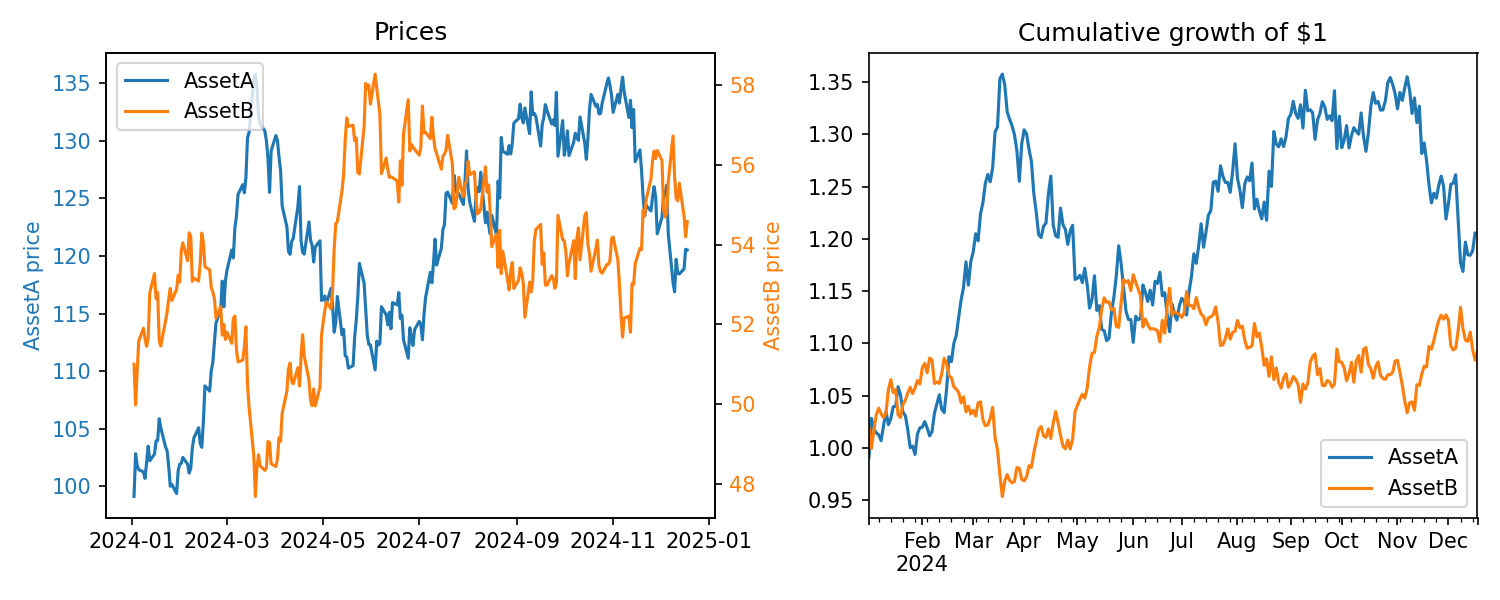
\includegraphics[width=\linewidth]{ch2_fig_prices_growth.png}
    \caption{Output of the code above: simulated AssetA and AssetB prices, each on its own y-axis (left), and the cumulative growth of \$1 invested in each, which shares a single axis since both series start at the same value (right), over a 252-day simulated price history.}
    \label{fig:ch2-prices-growth}
\end{figure}

Visualization is not merely decorative. It is part of the analytical process. A model may appear strong in a statistical summary, but a plot may reveal outliers, regime shifts, or data problems that would otherwise go unnoticed. In finance, where data quality and market context matter greatly, visualization is an essential discipline, and it is often the fastest way to notice that two return series are moving in opposite directions, as AssetA and AssetB do here.

Two other chart types are used constantly in financial analysis. A histogram of returns shows the shape of the return distribution, revealing skewness or heavy tails that summary statistics alone can obscure:

\begin{verbatim}
fig, ax = plt.subplots(figsize=(6, 4))
returns_viz["AssetA"].hist(ax=ax, bins=20)
ax.set_title("Distribution of AssetA daily returns")
ax.set_xlabel("Return")
plt.tight_layout()
\end{verbatim}

\begin{figure}[htbp]
    \centering
    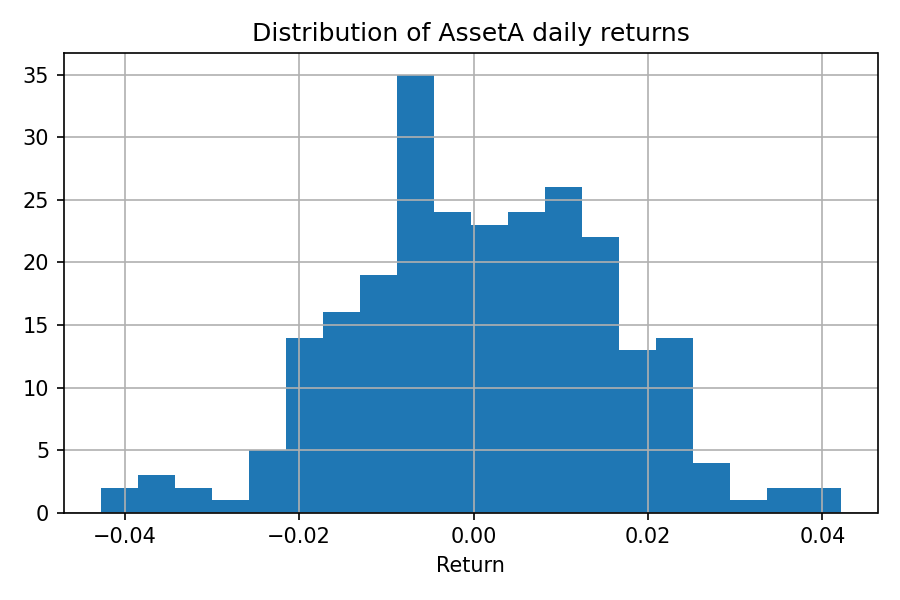
\includegraphics[width=0.7\linewidth]{ch2_fig_histogram.png}
    \caption{Output of the code above: the distribution of AssetA's simulated daily returns over the 252-day history. With hundreds of observations the shape is now informative, and the same code applied to real return data of any length would reveal skewness and heavy tails that summary statistics can miss.}
    \label{fig:ch2-histogram}
\end{figure}

A scatter plot of one asset's returns against another's is the most direct way to visualize a correlation like the one computed numerically in Section~\ref{sec:worked-example}:

\begin{verbatim}
fig, ax = plt.subplots(figsize=(5, 5))
ax.scatter(returns_viz["AssetA"], returns_viz["AssetB"], alpha=0.6)
ax.set_xlabel("AssetA return")
ax.set_ylabel("AssetB return")
ax.set_title(f"Correlation: {returns_viz['AssetA'].corr(returns_viz['AssetB']):.3f}")
plt.tight_layout()
\end{verbatim}

\begin{figure}[htbp]
    \centering
    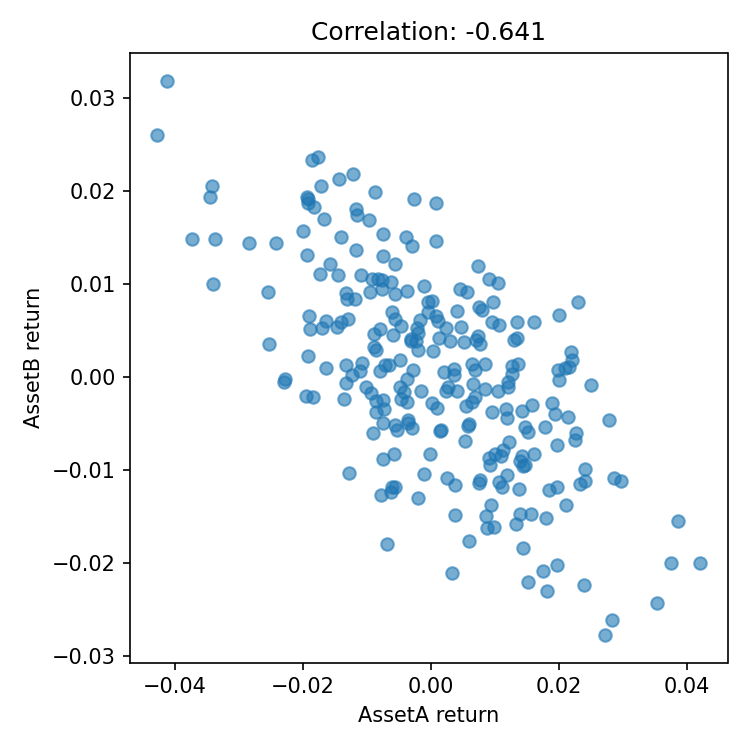
\includegraphics[width=0.55\linewidth]{ch2_fig_scatter.png}
    \caption{Output of the code above: simulated AssetA daily returns plotted against simulated AssetB daily returns. The cloud of points slopes visibly downward, consistent with the simulated correlation of $-0.641$.}
    \label{fig:ch2-scatter}
\end{figure}

Figure~\ref{fig:ch2-scatter} shows the cloud of 252 points sloping visibly downward, since a negative correlation means the two assets tend to move in opposite directions; with a real analysis, the same chart becomes a genuinely useful diagnostic for spotting nonlinear relationships or clusters that a single correlation number, a linear summary, cannot capture. The chapter's own four-observation example (Section~\ref{sec:worked-example}) shows the same qualitative pattern with an even stronger correlation of $-0.896$, but has too few points to plot informatively.

\section{Data Cleaning and Preparation}\index{Data Cleaning and Preparation}
\label{sec:data-cleaning}

Raw financial data often contains issues: missing entries, duplicate observations, outliers, inconsistent dates, or formatting errors. Data cleaning is therefore a major part of practical work. A well-designed pipeline may involve aligning multiple time series, filling missing observations carefully, adjusting for corporate actions such as dividends and splits, and removing clearly erroneous values.

Figure~\ref{fig:data_pipeline} shows a simple financial data workflow, and the code below shows a typical cleaning step: forward-filling a small gap in a price series (for example, caused by a data feed outage) rather than silently dropping the observation, which would misalign the two return series.

\begin{verbatim}
raw = prices.copy()
raw.loc["2024-01-04", "AssetB"] = np.nan  # simulate a missing quote
cleaned = raw.ffill()
print(raw["AssetB"].isna().sum(), "missing value(s) before cleaning")
print(cleaned["AssetB"].isna().sum(), "missing value(s) after cleaning")
# 1 missing value(s) before cleaning
# 0 missing value(s) after cleaning
\end{verbatim}

\begin{figure}[htbp]
    \centering
    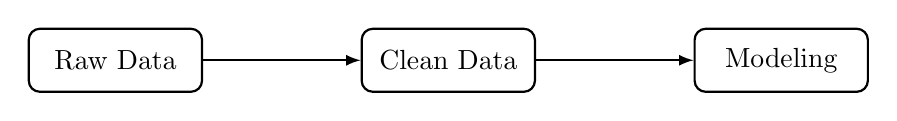
\begin{tikzpicture}[>=latex,thick,node distance=2.0cm]
        \node[draw,rounded corners,minimum width=2.2cm,minimum height=0.8cm] (raw) {Raw Data};
        \node[draw,rounded corners,minimum width=2.2cm,minimum height=0.8cm,right=of raw] (clean) {Clean Data};
        \node[draw,rounded corners,minimum width=2.2cm,minimum height=0.8cm,right=of clean] (model) {Modeling};
        \draw[->] (raw) -- (clean);
        \draw[->] (clean) -- (model);
    \end{tikzpicture}
    \caption{A typical financial data pipeline moves from raw data to cleaned inputs and then to modeling.}
    \label{fig:data_pipeline}
\end{figure}

Forward-filling is appropriate for a short gap in an otherwise liquid series, but it is not always the right choice: forward-filling an illiquid security for many consecutive days can create the false impression of zero volatility. A price series for a stock must also often be adjusted for splits and dividends to produce a consistent total return series; otherwise, the historical performance may be distorted by mechanical price drops that have nothing to do with economic losses. This is an important lesson for quantitative finance: even a sophisticated model is only as good as the data that feed it.

\section{A Worked Example: Building and Evaluating a Two-Asset Portfolio}\index{Building and Evaluating a Two-Asset Portfolio}
\label{sec:worked-example}

This section ties the chapter's running example together into a small but complete analysis, the kind of workflow an analyst repeats constantly, just at a larger scale. Suppose an analyst wants to evaluate an equally weighted portfolio of AssetA and AssetB.

\begin{verbatim}
weights = np.array([0.5, 0.5])
portfolio_returns = returns.dot(weights)
print(portfolio_returns.round(4))
# 2024-01-03    0.0150
# 2024-01-04    0.0026
# 2024-01-05    0.0123
# 2024-01-08    0.0052
# dtype: float64

port_mean = portfolio_returns.mean()
port_vol = portfolio_returns.std(ddof=1)
print(round(port_mean, 4), round(port_vol, 4))
# 0.0088 0.0058
\end{verbatim}

Compare the portfolio's volatility of 0.58\% to the weighted average of the two assets' individual volatilities, $0.5 \times 2.03\% + 0.5 \times 1.08\% = 1.56\%$. The portfolio is far less volatile than either asset alone, and much less volatile than a naive average of their volatilities would suggest. This is the diversification effect introduced conceptually in Chapter 1, and it can now be made precise. The covariance between the two return series is

\begin{verbatim}
cov_matrix = returns.cov()
print(cov_matrix.round(6))
#          AssetA    AssetB
# AssetA  0.000414 -0.000198
# AssetB -0.000198  0.000118

corr = returns.corr().iloc[0, 1]
print(round(corr, 3))
# -0.896
\end{verbatim}
so the two assets have a strong negative correlation of about $-0.90$. The variance of an equally weighted two-asset portfolio is given by
\begin{equation*}
\sigma_p^2 = w_A^2 \sigma_A^2 + w_B^2 \sigma_B^2 + 2 w_A w_B \sigma_{AB},
\end{equation*}
and substituting $w_A = w_B = 0.5$, $\sigma_A^2 = 0.000414$, $\sigma_B^2 = 0.000118$, and $\sigma_{AB} = -0.000198$ gives
\begin{equation*}
\sigma_p^2 = 0.25(0.000414) + 0.25(0.000118) + 2(0.25)(-0.000198) = 0.000034,
\end{equation*}
so $\sigma_p = \sqrt{0.000034} \approx 0.58\%$, exactly matching the value computed directly from the portfolio return series. This equivalence, between the formula and the code, is a useful checkpoint: whenever a hand-derived formula and a direct computation on the data disagree, there is a bug somewhere, either in the formula or in the code, and reconciling the two is one of the most valuable debugging habits a quantitative analyst can build.

The ability to conduct such analyses quickly, and to extend them immediately to many more assets and much longer histories, is one reason Python is widely used in finance. It allows researchers to iterate quickly, test ideas, and communicate results in a reproducible way. In a domain where decisions are often made under time pressure, this speed matters.

\section{Scaling Up: From Two Assets to a Small Portfolio Universe}\index{Scaling Up: From Two Assets to a Small Portfolio Universe}

The two-asset example above was deliberately small so that every number could be checked by hand. The code, however, is written in a way that scales to any number of assets without modification, which is worth demonstrating explicitly. Adding a third asset, AssetC, requires only adding a column to the original DataFrame:

\begin{verbatim}
prices["AssetC"] = [200.00, 198.00, 202.00, 199.00, 203.00]
returns3 = prices.pct_change().dropna()
print(returns3.round(4))
#             AssetA  AssetB  AssetC
# 2024-01-03  0.0200  0.0100 -0.0100
# 2024-01-04 -0.0098  0.0150  0.0202
# 2024-01-05  0.0297 -0.0051 -0.0149
# 2024-01-08 -0.0096  0.0200  0.0201
\end{verbatim}

Not a single line of the return, covariance, or portfolio-variance calculation needs to change; \texttt{pct\_change()}, \texttt{.cov()}, and matrix multiplication all operate the same way regardless of how many columns the DataFrame has:

\begin{verbatim}
weights3 = np.array([1/3, 1/3, 1/3])
port3 = returns3.dot(weights3)
print(port3.round(4))
# 2024-01-03    0.0067
# 2024-01-04    0.0085
# 2024-01-05    0.0033
# 2024-01-08    0.0102

cov3 = returns3.cov()
port_var3 = weights3 @ cov3.values @ weights3
print(f"Equal-weighted 3-asset portfolio volatility: {np.sqrt(port_var3):.4f}")
# Equal-weighted 3-asset portfolio volatility: 0.0030
\end{verbatim}

The expression \texttt{weights3 @ cov3.values @ weights3} is exactly the matrix form of the portfolio variance formula, $w^\top \Sigma w$, mentioned in Section 2.18, and it works identically whether $w$ has 2, 3, or 200 entries. This is the practical payoff of writing analysis code in terms of vectors and matrices rather than named variables for each individual asset: a script built this way for a two-asset illustration is already, without any rewriting, the same script a researcher would use on a portfolio of hundreds of securities, which is exactly the setting Chapter 10's portfolio optimization methods are built to handle.

\subsection*{Object-Oriented Programming: A Reusable \texttt{Portfolio} Class}\index{Object-Oriented Programming}

The procedural style used throughout this chapter, a sequence of variable assignments and function calls, works well for a single, one-off analysis, but repeating the same mean, volatility, and variance calculations for every new portfolio a researcher wants to evaluate invites exactly the kind of copy-paste duplication Section~\ref{sec:vectorization-performance}'s performance discussion and this chapter's reproducibility section both warn against. Object-oriented programming addresses this with a \texttt{class}: a template, defined once, that bundles a set of related data (here, a portfolio's returns and weights) together with the functions, called \emph{methods} when they belong to a class, that operate on that data, so that every new portfolio can be built from the same reusable blueprint instead of copying and re-editing the same calculations by hand each time:

\begin{verbatim}
class Portfolio:
    def __init__(self, returns, weights):
        self.returns = returns
        self.weights = weights

    @property
    def portfolio_returns(self):
        return self.returns.dot(self.weights)

    @property
    def mean(self):
        return self.portfolio_returns.mean()

    @property
    def volatility(self):
        return self.portfolio_returns.std(ddof=1)

    def variance_from_formula(self):
        cov = self.returns.cov().values
        return self.weights @ cov @ self.weights
\end{verbatim}

Instantiating this class on the same two-asset data used throughout the chapter reproduces every number already computed by hand,
\begin{verbatim}
portfolio = Portfolio(returns, weights)
print(round(portfolio.mean, 4), round(portfolio.volatility, 4))
# 0.0088 0.0058
print(round(portfolio.variance_from_formula(), 6))
# 3.4e-05
\end{verbatim}
but the real payoff appears when evaluating the three-asset portfolio built above: \texttt{Portfolio(returns3, weights3)} produces the correct mean, volatility, and formula-based variance for the three-asset case using the identical class definition, with no new code written at all. This is precisely what ``scaling up'' means in an object-oriented codebase: the \texttt{Portfolio} class is a single, tested abstraction that every future portfolio, of any size, can reuse, rather than a script that must be copied and re-edited each time a new set of assets needs evaluating, exactly the kind of reusable component a production research or trading system is built from.

\section{Working with Time Series and Financial Data}\index{Working with Time Series and Financial Data}

Many financial datasets are time series, meaning that observations are indexed by time and ordered sequentially. Stock prices, interest rates, exchange rates, and macroeconomic indicators all arrive as time-dependent data. Working with such data requires careful handling of date indexes, alignment, and missing observations. In Python, pandas is particularly useful because it provides a time-indexed data structure that makes these operations natural, including resampling to a different frequency and computing rolling statistics:

\begin{verbatim}
rolling_vol = returns["AssetA"].rolling(window=2).std()
print(rolling_vol.round(4))
# 2024-01-03       NaN
# 2024-01-04    0.0211
# 2024-01-05    0.0279
# 2024-01-08    0.0278
# dtype: float64
\end{verbatim}

A common workflow is to import historical prices, convert them into a time series, compute returns, and then study autocorrelation, volatility clustering, and trends. These steps are essential because many financial models depend on the idea that the future is not independent of the past. Yet the time dependence in financial data is often subtle and nonstationary, which makes careful analysis, and the topics of Chapter 7, necessary.

\section{Why Vectorization Matters: A Performance Comparison}\index{Why Vectorization Matters: A Performance Comparison}
\label{sec:vectorization-performance}

Section~\ref{sec:vectorization} claimed that vectorized array operations are faster than an equivalent Python-level loop; it is worth demonstrating this claim rather than only asserting it. Consider computing the cumulative growth of \$1 across 100,000 simulated daily returns, once with an explicit loop and once with NumPy's vectorized \texttt{cumprod}:

\begin{verbatim}
import time

rng = np.random.default_rng(0)
simulated_returns = rng.normal(0.0005, 0.01, 100_000)

start = time.perf_counter()
total = 1.0
loop_values = []
for r in simulated_returns:
    total *= (1 + r)
    loop_values.append(total)
loop_time = time.perf_counter() - start

start = time.perf_counter()
vectorized_values = np.cumprod(1 + simulated_returns)
vector_time = time.perf_counter() - start

print(f"Loop: {loop_time:.4f}s, Vectorized: {vector_time:.4f}s, "
      f"speedup: {loop_time/vector_time:.0f}x")
# Loop: 0.0394s, Vectorized: 0.0010s, speedup: 39x
\end{verbatim}

Both approaches produce identical final values, since they compute the same mathematical quantity, but the vectorized version is roughly 39 times faster on this test (the exact figure is machine-dependent and will vary, but a factor of 10 to 100 is typical for this kind of calculation). The reason is that the Python-level loop pays interpreter overhead, argument checking, dynamic type dispatch, on every single one of the 100,000 iterations, while \texttt{cumprod} executes the equivalent loop once, in compiled C code, over contiguous memory. This gap widens, not narrows, as the dataset grows, which is precisely why Section 2.20's discussion of performance at scale emphasizes vectorized NumPy and pandas operations as the default approach, reserving explicit loops for calculations, like the sequential compounding example in Section 2.4, that are genuinely path-dependent and cannot be vectorized.

\section{Handling Errors and Common Pitfalls}\index{Handling Errors and Common Pitfalls}

Financial data pipelines fail constantly, in small, mundane ways: a data feed returns a missing value, a ticker is misspelled, a division produces infinity because a denominator was zero. Python's \texttt{try}/\texttt{except} block lets a program catch such errors and respond deliberately rather than crashing outright:

\begin{verbatim}
def safe_return(price_now, price_before):
    try:
        return (price_now - price_before) / price_before
    except ZeroDivisionError:
        return float("nan")

print(safe_return(105.0, 100.0))
# 0.05
print(safe_return(105.0, 0.0))
# nan
\end{verbatim}

Returning \texttt{nan} (not-a-number) rather than letting the program crash allows downstream code, and pandas in particular, to continue processing the rest of a dataset while clearly marking the problematic observation, exactly like the missing-value handling in Section~\ref{sec:data-cleaning}. A few pitfalls recur often enough in financial Python code to be worth naming explicitly:

\begin{itemize}
    \item \textbf{Silent \texttt{NaN} propagation.} Almost any arithmetic operation involving \texttt{NaN} produces another \texttt{NaN} rather than an error, so a single bad data point can silently spread through an entire calculation (a covariance matrix, for example) without any visible warning.
    \item \textbf{Comparing floating-point numbers for exact equality.} Because of how computers represent decimal numbers, a calculation that should mathematically equal \texttt{0.3} may instead equal \texttt{0.30000000000000004}; use a tolerance-based comparison (\texttt{np.isclose}) rather than \texttt{==} when checking floating-point results.
    \item \textbf{Mutating a DataFrame while iterating over it.} Modifying rows of a DataFrame inside a loop over that same DataFrame can produce confusing, order-dependent results; it is almost always better to build a new column or DataFrame with a vectorized expression instead.
    \item \textbf{Off-by-one errors in lagged calculations.} Return, rolling-window, and lag calculations are especially prone to off-by-one mistakes, using today's price where yesterday's was intended, which can silently introduce look-ahead bias into a backtest, the same problem discussed in Section 2.20.
\end{itemize}

\section{Descriptive Statistics and Portfolio Analytics}\index{Descriptive Statistics and Portfolio Analytics}

Once data are imported and cleaned, Python can be used to calculate descriptive statistics such as averages, standard deviations, skewness, and kurtosis. These statistics summarize the distribution of returns and provide a starting point for risk analysis:

\begin{verbatim}
summary = returns.describe().round(4)
print(summary)
#        AssetA  AssetB
# count  4.0000  4.0000
# mean   0.0076  0.0100
# std    0.0203  0.0108
# min   -0.0098 -0.0051
# 25%   -0.0097  0.0062
# 50%    0.0052  0.0125
# 75%    0.0224  0.0163
# max    0.0297  0.0200
\end{verbatim}

For a portfolio, one may also compute correlations between assets, covariance matrices, and portfolio volatility, exactly as in the worked example above. These quantities are central to diversification and asset allocation, and they generalize directly to portfolios with many assets: with $n$ assets, weights $w \in \mathbb{R}^n$, and covariance matrix $\Sigma$, portfolio variance is $\sigma_p^2 = w^\top \Sigma w$, which is precisely the two-asset formula written in matrix form.

The advantage of Python here is that the same code applies unchanged whether there are 2 assets or 200. A single script can compute rolling volatilities, drawdowns, and Sharpe-like performance measures across a whole universe of securities. This efficiency is crucial when a researcher wants to compare strategies, evaluate risk, or test whether a signal remains useful after transaction costs.

\section{Reproducibility, Version Control, and Good Practice}\index{Reproducibility, Version Control, and Good Practice}

One of the most important lessons in computational finance is that analysis must be reproducible. A model or result that cannot be rerun by another analyst, or by the same analyst six months later, is of limited value. Python supports reproducibility through scripts, notebooks, and package management. A clear workflow includes:

\begin{itemize}
    \item Recording exact package versions, for example in a \texttt{requirements.txt} or \texttt{environment.yml} file, so that a colleague (or a future you) can recreate the same environment.
    \item Saving raw data separately from cleaned or derived data, so that a cleaning step can be re-run or audited without re-fetching from the original source.
    \item Documenting transformations, ideally in code and comments rather than in a separate document that can drift out of sync with the script.
    \item Separating analysis from presentation, so that a notebook used to explore an idea is not the same artifact used to report a result to a manager or regulator.
    \item Using version control (such as Git) to track changes to code over time, including the ability to identify exactly which version of the code produced a given historical result.
    \item Fixing random seeds (as in \texttt{np.random.default\_rng(0)} in Section~\ref{sec:vectorization-performance}) whenever a calculation involves simulation, so that two runs of the same script on the same data produce identical results rather than only similar ones.
    \item Writing small checks directly into a script or notebook, such as the put-call parity check used in Chapter 5 or the accounting-identity check used in Chapter 4, so that a silent bug is caught immediately rather than discovered much later when it has already propagated into a report or a trading decision.
\end{itemize}

\subsection*{Unit Testing: Making Checks Automatic}\index{Unit Testing}

The ``small checks'' in the list above become far more valuable once they are written as an actual, automatically run test rather than a one-off \texttt{print} statement an analyst has to remember to inspect. A unit test is simply a function that exercises a piece of code and uses Python's \texttt{assert} statement to fail loudly if the result is not what is expected. Section~\ref{sec:worked-example}'s own observation, that the portfolio-variance formula and the direct computation from the return series agree, is exactly the kind of invariant worth encoding this way:

\begin{verbatim}
def test_portfolio_variance_matches_formula():
    weights = np.array([0.5, 0.5])
    cov = returns.cov().values
    var_A, var_B, cov_AB = cov[0, 0], cov[1, 1], cov[0, 1]
    formula_variance = (
        weights[0]**2 * var_A + weights[1]**2 * var_B + 2 * weights[0] * weights[1] * cov_AB
    )
    direct_variance = returns.dot(weights).var(ddof=1)
    assert abs(formula_variance - direct_variance) < 1e-10, \
        "Portfolio variance formula does not match direct computation!"
    print("Test passed: formula-based and direct portfolio variance agree.")

test_portfolio_variance_matches_formula()
# Test passed: formula-based and direct portfolio variance agree.
\end{verbatim}

The specific tolerance, $10^{-10}$, matters: it is loose enough to absorb ordinary floating-point rounding but tight enough to catch a genuine error, for example an accidentally transposed covariance term or a forgotten factor of two on the cross term, exactly the kind of subtle bug this book's own notebooks have caught in earlier chapters (Chapter 11's \texttt{statistics.mean} silent-truncation bug is a real example of precisely this failure mode). A single test like this one costs a few lines to write and runs in a fraction of a second, but it converts a fact an analyst has verified once, by hand, into a fact that is re-verified automatically every single time the surrounding code changes, catching a regression immediately rather than only when a downstream number looks suspicious. Production financial codebases typically collect dozens or hundreds of such tests, run automatically before any code change is accepted, using a dedicated testing framework such as \texttt{pytest} rather than calling test functions manually as shown here, but the underlying principle, encode a known-correct result as an executable check rather than a comment, is exactly the same at any scale.

Reproducibility is not a bureaucratic nicety layered on top of the real analytical work; in a financial setting it is frequently a legal and professional requirement. A regulator investigating a trading loss, an auditor reviewing a valuation, or a portfolio manager questioning a backtested strategy will all expect to be able to trace a reported number back to the exact code and data that produced it. A workflow that cannot support this kind of retrospective scrutiny is a liability regardless of how sophisticated its underlying models are.

Good practice also means writing code that is understandable. Financial projects often involve several collaborators, long time horizons, and changing requirements. A readable function, a clear variable name, and a documented transformation can prevent errors and make the analysis easier to audit. In a regulated environment, this discipline is not optional; it is a professional necessity, since a regulator or auditor may ask exactly how a number was produced months or years after the fact.

\section{Challenges in Applying Python to Financial Data}

Several practical challenges arise repeatedly when Python is used for financial analysis, and they are worth naming explicitly before moving on to statistical and machine learning methods.

\textbf{Data quality and vendor discrepancies.} Different data vendors can report slightly different prices, adjust for corporate actions differently, or use different conventions for holidays and time zones. A workflow that silently trusts a single source can propagate vendor-specific errors into every downstream result.

\textbf{Look-ahead and survivorship bias.} It is easy to accidentally use information that would not have been available at the time of a decision, for example by using a company's current list of index constituents to study its past performance, which silently excludes firms that were delisted or went bankrupt. Both issues can make a backtest look far more profitable than any strategy could actually have been in real time.

\textbf{Non-stationarity and changing data schemas.} Return distributions, volatility regimes, and even the format of vendor data feeds change over time. Code written for one period's data conventions may silently produce wrong answers, rather than an error, when applied to a later period with a slightly different schema.

\textbf{Performance at scale.} A script that works well on five days of data for two assets, as in this chapter's example, may become far too slow when applied to years of tick-by-tick data across thousands of instruments. Vectorized NumPy and pandas operations help, but some tasks genuinely require more specialized tools, such as columnar file formats, database systems, or distributed computing frameworks.

\textbf{Environment and dependency drift.} A notebook that runs correctly today may fail in a year if underlying libraries change their behavior or drop support for older syntax. This is why pinning dependency versions and periodically re-validating old code are standard practice in production financial systems.

\textbf{Latency and real-time constraints.} Some applications, particularly in trading, require code to execute within milliseconds or microseconds. Python's convenience often comes at the cost of raw execution speed, which is why performance-critical components are sometimes implemented in compiled languages or accelerated with tools such as Numba or Cython, while Python remains the layer used for research, orchestration, and analysis.

\textbf{Dependency and library version conflicts.} A pandas or NumPy upgrade can silently change the default behavior of a function (for example, how missing values are handled in an aggregation), which means code that has not been re-tested against a new library version should not be assumed to still behave identically, even if it runs without raising an error.

\textbf{The gap between exploratory and production code.} Code written quickly in a notebook to explore an idea is rarely suitable, unmodified, for a system that will run unattended in production; exploratory code typically lacks the error handling, logging, and automated testing that a production financial system requires, and treating the two as interchangeable is a common source of operational incidents.

\section{Key Takeaways}

Python is a practical and powerful tool for financial analysis because it supports efficient computation, flexible data handling, and reproducible workflows. The libraries in the Python ecosystem make it possible to move from raw market data to descriptive analysis, forecasting, and machine learning. The chapter's worked example showed how a handful of pandas and NumPy operations, applied to just five days of prices, can reveal a meaningful diversification effect and how a formula derived on paper should match a direct computation on the data. For readers who aim to apply AI in finance, Python is not optional; it is a core capability, and the habits introduced here, vectorized computation, careful data cleaning, and reproducible workflows, scale directly to the much larger datasets used in later chapters.

A few distinctions from this chapter are worth restating because they recur, largely unchanged, in every later chapter. First, the choice between a loop and a vectorized operation is not a stylistic preference; it is a question of whether a calculation is independent across observations (vectorize it) or genuinely sequential, like the compounding balance example (a loop, or an equivalent closed-form formula, is required). Second, combining data from multiple sources, the \texttt{merge} and \texttt{groupby} operations in Section 2.10, is not a peripheral skill but a central one, since almost no real financial analysis works from a single, already-tidy table. Third, every code example in this chapter was written to be checked, either by hand, as with the four AssetA and AssetB returns, or by running the companion notebook and comparing outputs line by line; this habit of verifying rather than trusting a computation is exactly the discipline that later chapters rely on when the calculations become too complex to check by hand at all, such as the maximum-likelihood-estimated GARCH model\index{GARCH model}s in Chapter 7 or the gradient-boosted trees in Chapter 6.

\section{Suggested Exercises}

\begin{enumerate}
    \item Write a Python function that computes the future value of an investment given a price, an annual rate, and a number of years, and use it to verify the two examples in Section~\ref{sec:first-session}.
    \item Recreate the \texttt{prices} DataFrame from Section 2.5, add a third asset, \texttt{AssetC}, with your own five prices, and compute its returns using \texttt{pct\_change()}.
    \item Using the covariance formula for portfolio variance, compute the volatility of a portfolio with weights 0.7 on AssetA and 0.3 on AssetB, and check your answer against a direct computation on \texttt{portfolio\_returns}.
    \item Modify the data-cleaning example to simulate two consecutive missing values in AssetB, apply forward-fill, and discuss whether this is still a reasonable choice.
    \item Plot the cumulative growth of \$1 invested in AssetA, AssetB, and the equally weighted portfolio on the same chart, and describe what the chart shows about diversification that the summary statistics alone do not.
    \item Explain why a positive correlation between two assets would change the diversification benefit computed in Section~\ref{sec:worked-example}, and recompute the portfolio volatility assuming a correlation of $+0.90$ instead of $-0.896$, holding the individual volatilities fixed.
    \item Describe one concrete situation in which look-ahead bias could enter a Python backtesting script without the analyst noticing, and propose a coding practice that would prevent it.
    \item Rewrite the \texttt{classify\_return} function from Section 2.4 as a single list comprehension using a conditional expression, and verify it produces the same labels for the four AssetA returns.
    \item Using \texttt{np.select} as in Section 2.8, classify AssetB's four returns into ``strong gain'' ($>1\%$), ``small gain'' ($>0\%$), ``flat,'' or ``loss,'' and compare the result to AssetA's classification.
    \item Extend the \texttt{securities\_df} and \texttt{shares} example in Section 2.10 with one more security of your choosing, recompute \texttt{position\_value}, and recompute the sector summary.
    \item Extend the \texttt{extended\_prices} series in Section 2.10 with five more business days of your own prices, and resample the full series to weekly frequency using both \texttt{.last()} and \texttt{.mean()}; explain when each aggregation would be the more appropriate choice.
    \item Using the pattern in Section~\ref{sec:vectorization-performance}, describe (without necessarily running the code) why a loop that appends to a Python list one element at a time is typically slower than pre-allocating a NumPy array and filling it by index, even though both avoid calling a vectorized function.
    \item Using this chapter's \texttt{Portfolio} class, instantiate it with weights $0.7$ on AssetA and $0.3$ on AssetB, and verify that \texttt{portfolio.volatility} matches the answer you computed by hand in Exercise 3.
    \item Add a second unit test, \texttt{test\_weights\_sum\_to\_one}, that asserts a portfolio's weights sum to $1.0$ within a small tolerance, and explain what kind of real coding mistake this test would catch that the variance-formula test would not.
\end{enumerate}

\section{Further Reading}

\begin{itemize}
    \item McKinney, \emph{Python for Data Analysis}. Written by pandas' original author, this is the definitive reference for the DataFrame, groupby, merge, and resample operations introduced in this chapter, covering many more edge cases and options than a single chapter can.
    \item VanderPlas, \emph{Python Data Science Handbook}. A broader tour of NumPy, pandas, and visualization that fills in the general-purpose Python and data-science background this chapter assumes, alongside its finance-specific examples.
    \item Hilpisch, \emph{Python for Finance}. Extends this chapter's two-asset portfolio example toward the derivatives pricing, risk management, and algorithmic trading applications covered later in this book, using the same core pandas and NumPy toolkit.
    \item Hilpisch, \emph{Python for Algorithmic Trading}. A practical, code-heavy treatment of building and backtesting trading systems in Python, a natural next step after this chapter's vectorization and performance material for readers headed toward Chapters 11 and 12.
\end{itemize}

\end{document}
